%%%%%%%%%%%%%%%%%%%%%%%%%%%%%%%%%%%%%%%%%
% Short Sectioned Assignment LaTeX Template Version 1.0 (5/5/12)
% This template has been downloaded from: http://www.LaTeXTemplates.com
% Original author:  Frits Wenneker (http://www.howtotex.com)
% License: CC BY-NC-SA 3.0 (http://creativecommons.org/licenses/by-nc-sa/3.0/)
%%%%%%%%%%%%%%%%%%%%%%%%%%%%%%%%%%%%%%%%%

%----------------------------------------------------------------------------------------
%	PACKAGES AND OTHER DOCUMENT CONFIGURATIONS
%----------------------------------------------------------------------------------------

\documentclass[paper=a4, fontsize=11pt]{scrartcl} % A4 paper and 11pt font size

% ---- Entrada y salida de texto -----

\usepackage[T1]{fontenc} % Use 8-bit encoding that has 256 glyphs
\usepackage[utf8]{inputenc}
%\usepackage{fourier} % Use the Adobe Utopia font for the document - comment this line to return to the LaTeX default

% ---- Idioma --------

\usepackage[spanish, es-tabla]{babel} % Selecciona el español para palabras introducidas automáticamente, p.ej. "septiembre" en la fecha y especifica que se use la palabra Tabla en vez de Cuadro

% ---- Otros paquetes ----

\usepackage{url} % ,href} %para incluir URLs e hipervínculos dentro del texto (aunque hay que instalar href)
\usepackage{amsmath,amsfonts,amsthm} % Math packages
%\usepackage{graphics,graphicx, floatrow} %para incluir imágenes y notas en las imágenes
\usepackage{graphics,graphicx, float} %para incluir imágenes y colocarlas
\usepackage{epstopdf}

% Para hacer tablas comlejas
%\usepackage{multirow}
%\usepackage{threeparttable}

%\usepackage{sectsty} % Allows customizing section commands
%\allsectionsfont{\centering \normalfont\scshape} % Make all sections centered, the default font and small caps

\usepackage{fancyhdr} % Custom headers and footers
\pagestyle{fancyplain} % Makes all pages in the document conform to the custom headers and footers
\fancyhead{} % No page header - if you want one, create it in the same way as the footers below
\fancyfoot[L]{} % Empty left footer
\fancyfoot[C]{} % Empty center footer
\fancyfoot[R]{\thepage} % Page numbering for right footer
\renewcommand{\headrulewidth}{0pt} % Remove header underlines
\renewcommand{\footrulewidth}{0pt} % Remove footer underlines
\setlength{\headheight}{13.6pt} % Customize the height of the header

\numberwithin{equation}{section} % Number equations within sections (i.e. 1.1, 1.2, 2.1, 2.2 instead of 1, 2, 3, 4)
\numberwithin{figure}{section} % Number figures within sections (i.e. 1.1, 1.2, 2.1, 2.2 instead of 1, 2, 3, 4)
\numberwithin{table}{section} % Number tables within sections (i.e. 1.1, 1.2, 2.1, 2.2 instead of 1, 2, 3, 4)

\setlength\parindent{0pt} % Removes all indentation from paragraphs - comment this line for an assignment with lots of text

\newcommand{\horrule}[1]{\rule{\linewidth}{#1}} % Create horizontal rule command with 1 argument of height


%----------------------------------------------------------------------------------------
%	TÍTULO Y DATOS DEL ALUMNO
%----------------------------------------------------------------------------------------


\title{	
\normalfont \normalsize 
\textsc{\textbf{Curso 2016-2017} \\ Grado en Ingeniería Informática \\ Universidad de Granada} \\ [25pt] % Your university, school and/or department name(s)
\horrule{0.5pt} \\[0.4cm] % Thin top horizontal rule
\huge Práctica 2: Algoritmo A* \\ % The assignment title
\horrule{2pt} \\[0.5cm] % Thick bottom horizontal rule
}

\author{Carlos Manuel Sequí Sánchez} % Nombre y apellidos

\date{\normalsize\today} % Incluye la fecha actual

%----------------------------------------------------------------------------------------
% DOCUMENTO
%----------------------------------------------------------------------------------------




\begin{document}

\maketitle % Muestra el Título

\newpage %inserta un salto de página

\tableofcontents % para generar el índice de contenidos

\listoffigures

\newpage

\section{Resumen inicial}

Para la resolución de la práctica he realizado todos los puntos que se piden en el guión, incluida la optimización. \\
Primeramente he realizado el algoritmo A* ordenando los nodos que se meten en la lista de abiertos con un functor, después he terminado de rellenar el método addNeighborCellsToOpenList para que se completasen todos los datos de un nuevo nodo.\\ Tras esto he procedido a implementar el camino más seguro haciendo uso de la función getCost del costmap. \\ Más tarde hice la optimización mediante pesos para elegir caminos de forma más rápida y, por último, los experimentos tomando medidas de metros recorridos, tiempo tomado y nodos expandidos. \\

\section{Creación del A*}

El algoritmo inicial era claramente una búsqueda en anchura, la cual exploraba todos los nodos que rodeaban al robot. Para pasarlo a una búsqueda con algoritmo A* lo único que hice fue cambiar los contenedores ''list'' por contenedores ''set'' de la STL y crearme mi propio functor (CMP) para usarlo con el ''set'' y que a la hora de insertar nuevos nodos en la openList en el método addNeighborCellsToOpenList se ordenasen de forma automática por orden creciente de fCost. \\ Además del orden de los nodos por fCost, también hubo que terminar de implementar el método addNeighborCellsToOpenList de manera que se completasen todos los campos de los nodos que se iban a añadir a la openList (faltaban por completar los campos gCost, hCost y fCost). \\
También he tenido en cuenta la conservación de los mejores padres comparando en toda iteración los nodos generados y que además ya están en abiertos con los nodos que hay en abiertos, es decir, una vez generados los nodos hijo, vemos los que ya están en la lista de abiertos y, en caso de que el gCost del padre de estos sea mejor que los de la openList, actualizamos dichos valores en los nodos de la lista de abiertos. \\

\section{Implementación del camino más seguro}

Para dicho propósito traté de utilizar la función footPrint implementada en el código proporcionado en la página web pero, tras comprobar y consultar con el profesor que la variable world\_model\_ daba problemas de enlazado a la hora de ejecutarse, decidí utilizar la función getCost del costmap, la cuál nos da información acerca de la proximidad que tiene una celda a un obstáculo. \\
Esta proximidad nos la da en un número del 0 al 255, de manera que cuanto más alto sea el valor devuelto por dicha función, más próxima se encuentra la celda a un obstáculo. \\
Sabiendo esto es fácil hacer uso de ella, pues nos basta con sumar el valor que devuelve la función al fCost, de manera que para celdas cercanas a obstáculos, el valor de fCost sea mayor y por tanto, la celda afectada tenga menor probabilidad de ser escogida que otra celda con menor valor de fCost. \\
Como podemos observar en la siguiente comparación a la izquierda (a) el camino creado está ligeramente más próximo a los obstáculos que el camino de la derecha(b), el cuál ha sido implementado con la función getCost del costmap.

\begin{figure}[H] %con el [H] le obligamos a situar aquí la figura
	\centering
	\subfigure[Camino menos seguro]{\includegraphics[scale=0.266]{./comparacionGetCost1/1}}
	\subfigure[Camino más seguro]{\includegraphics[scale=0.322]{./comparacionGetCost1/2}}
\end{figure}

A continuación un ejemplo aún más claro del uso de esta función. Como vemos en las siguientes figuras, el robot es incluso capaz de decidir si un camino es demasiado peligroso como para tomarlo o no. En la figura (c) podemos ver como pasa por un estrecho, poniéndose en peligro por el hecho de que podría impactar con algún obstáculo. En la figura (d) podemos ver como gracias a la implementación realizada con el getCost el robot no se la juega a pasar por un camino tan estrecho y escoge uno alternativo mucho más seguro.

\begin{figure}[H] %con el [H] le obligamos a situar aquí la figura
	\centering
	\subfigure[Camino menos seguro]{\includegraphics[scale=0.320]{./comparacionGetCostYCamino1/1}}
	\subfigure[Camino más seguro]{\includegraphics[scale=0.236]{./comparacionGetCostYCamino1/2}}
\end{figure}



\section{Optimización del algoritmo}

Para la optimización del algoritmo he tenido en cuenta el método por pesos explicado en las clases de teoría, el cual se basa en crear una relación (peso) entre la distancia que hay de la posición inicial donde se encuentra el robot y la posición del goal (distanciaInicioGoal) y la distancia que hay entre el nodo que esta siendo evaluado y el goal (distanciaNodoGoal), de manera que nos queda lo siguiente:

\[
	Peso = \frac{distanciaNodoGoal}{distanciaInicioGoal}
\]

Una vez obtenido dicho peso para cada uno de los nodos evaluados (en cada iteración) simplemente lo multiplicamos por el valor de fCost, de manera que cuanto más lejos se encuentre el nodo evaluado, mayor sera el valor del peso, por lo que también será mayor el valor del fCost y por tanto, tendrá menos prioridad a la hora de ser escogido para seguir expandiendo por ahí. Este método de optimización hace que se encuentren planes mucho antes que sin la mejora como veremos en las experimentaciones a continuación. Este es el ejemplo más claro que he logrado conseguir para mostrar la optimización del algoritmo. En el caso (a) tenemos un camino muy costoso con un tiempo de cálculo de 111 segundos (c) y en el caso (b) tenemos un camino muy poco costoso con un tiempo de cálculo de 2.8 segundos (d), una mejora muy sustancial sin lugar a dudas.


\begin{figure}[H] %con el [H] le obligamos a situar aquí la figura
	\centering
	\subfigure[Camino más costoso]{\includegraphics[scale=0.28]{./camino5/1}}
	\subfigure[Camino menos costoso]{\includegraphics[scale=0.19]{./camino5/2}}
	\subfigure[Camino más costoso]{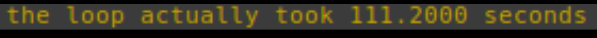
\includegraphics[scale=0.45]{./camino5/tiempoAntiguo}}
	\subfigure[Camino menos costoso]{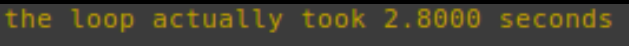
\includegraphics[scale=0.4]{./camino5/mejoraCamino5Tiempo}}
	\subfigure[Distancia recorrida: 65 metros]{
\includegraphics[scale=0.64]{./camino5/d5}}
	\subfigure[537 nodos recorridos en el algoritmo optimizado]{
\includegraphics[scale=0.6]{./5}}
\end{figure}



\newpage




\section{Experimento 1}

En este primer experimento podemos observar tanto el origen como el destino en la figura (a), cuyo recorrido tardó en ser calculado 5.7 segundos con un costo de 54.77 metros. El robot tuvo que recalcular la ruta 2 veces debido a que se dió cuenta de que no podía pasar por ciertos sitios:
la primera vez (figura (b)) tardo 5.9 segundos en recalcularla y la segunda (figura(c)) tardó 1.3 segundos con un costo de 22.7 metros de distancia hasta el destino.\\
La figura (e) es el tiempo de cálculo que gastó pensando la ruta con el algoritmo optimizado. Esta vez solo tuvo que recalcular una vez la ruta (a la misma altura de donde se encuentra el robot en la figura (c)) y ni tan siquiera apareció el tiempo que tardó en hacerlo por pantalla. Mostramos los nodos recorridos en los dos cálculos realizados con la optimización (figuaras h e i).

\begin{figure}[H] %con el [H] le obligamos a situar aquí la figura
	\centering
	\subfigure[Cálculo 1]{\includegraphics[scale=0.19]{./camino2/1}}
	\subfigure[Cálculo 2]{\includegraphics[scale=0.20]{./camino2/2}}
	\subfigure[Cálculo 3]{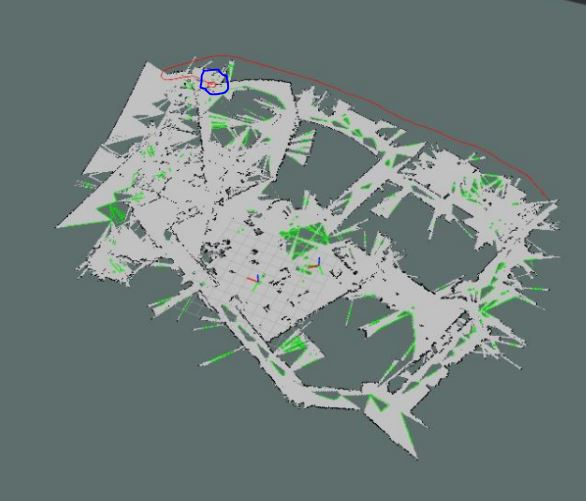
\includegraphics[scale=0.20]{./camino2/3}}
	\subfigure[Tiempos de cálculo]{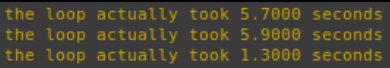
\includegraphics[scale=0.7]{./camino2/t1}}
	\subfigure[Tiempo mejorado de cálculo (con pesos)]{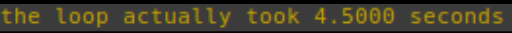
\includegraphics[scale=0.5]{./camino2/t2}}
	\subfigure[Distancia 1 = 54.77 metros]{
\includegraphics[scale=0.7]{./camino2/d21}}
	\subfigure[Distancia 2 = 22.70 metros]{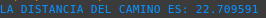
\includegraphics[scale=0.7]{./camino2/d22}}
	\subfigure[467 nodos recorridos en el cálculo 1]{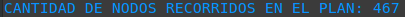
\includegraphics[scale=0.6]{./21}}
	\subfigure[189 nodos recorridos en el cálculo 2]{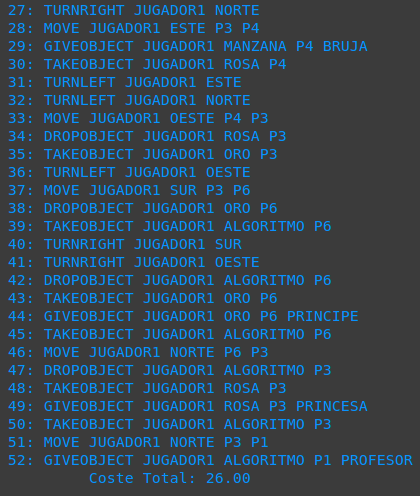
\includegraphics[scale=0.6]{./22}}
\end{figure}

\newpage


\section{Experimento 2}

En este experimento no obtuve mejoras ni en el tiempo de cálculo del recorrido ni en el propio recorrido, así que simplemente expongo el experimento con la figura (h) mostrando como el robot avanza hacia el objetivo y con la figura (i) mostrando como ha llegado ya al destino (arriba a la izquierda el punto rojo).\\

El tiempo de cálculo usado para este caso ha sido un total de 6 segundos y, la distancia recorrida en metros es de 65.9.

\begin{figure}[H] %con el [H] le obligamos a situar aquí la figura
	\centering
	\subfigure[Cálculo 1]{\includegraphics[scale=0.33]{./camino3/1}}
	\subfigure[Cálculo 2]{\includegraphics[scale=0.33]{./camino3/2}}
	\subfigure[Tiempo de cálculo = 6 segundos]{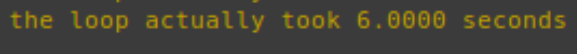
\includegraphics[scale=0.7]{./camino3/t3}}
	\subfigure[Distancia = 65.93 metros]{
\includegraphics[scale=1.2]{./camino3/d3}}
	\subfigure[537 nodos recorridos]{
\includegraphics[scale=1]{./5}}
	
\end{figure}
\newpage

\section{Experimento 3}

Este es el último experimento realizado. En las siguientes figuras muestro tanto el inicio (figura(l)) como el final (figura (m)) del recorrido calculado por el robot en la zona izquierda del mapa completo. \\
No pongo ningún tiempo porque el cálculo del recorrido ha sido instantáneo, es decir, al indicar el recorrido que quería que hiciese el robot, no ha aparecido el tiempo en pantalla ni tan siquiera. \\
La distancia recorrida es de 41 metros

\begin{figure}[H] %con el [H] le obligamos a situar aquí la figura
	\centering
	\subfigure[Inicio del recorrido]{\includegraphics[scale=0.33]{./camino4/1}}
	\subfigure[Final del recorrido]{\includegraphics[scale=0.39]{./camino4/2}}
	\subfigure[Distancia = 41 metros]{
\includegraphics[scale=1.2]{./camino4/d4}}
	\subfigure[345 nodos recorridos]{
\includegraphics[scale=1]{./4}}
\end{figure}

%------------------------------------------------




\end{document}
